\documentclass[12pt, letterpaper, fleqn]{report}
\usepackage[hidelinks]{hyperref}
\usepackage{geometry}
\usepackage{graphicx}
\usepackage{fix-cm}

\geometry{letterpaper, total={210mm,297mm}, left=20mm, right=20mm, top=20mm, bottom=20mm}

% Font size convention for this document:

% UI element : \textsl{name of the UI element}
% Nomenclature: ``name of the term defined''

\begin{document}

\begin{titlepage}
\begin{center}

% http://www.tex.ac.uk/cgi-bin/texfaq2html?label=fontsize

\textbf{\fontfamily{phv}\fontsize{30}{36}\selectfont USER MANUAL}\\[1.0cm]
\textbf{\fontfamily{phv}\fontsize{30}{36}\selectfont AND}\\[1.0cm]
\textbf{\fontfamily{phv}\fontsize{30}{36}\selectfont TECHNICAL DOCUMENTATION}\\[1.0cm]
\textbf{\fontfamily{phv}\fontsize{30}{36}\selectfont FOR}\\

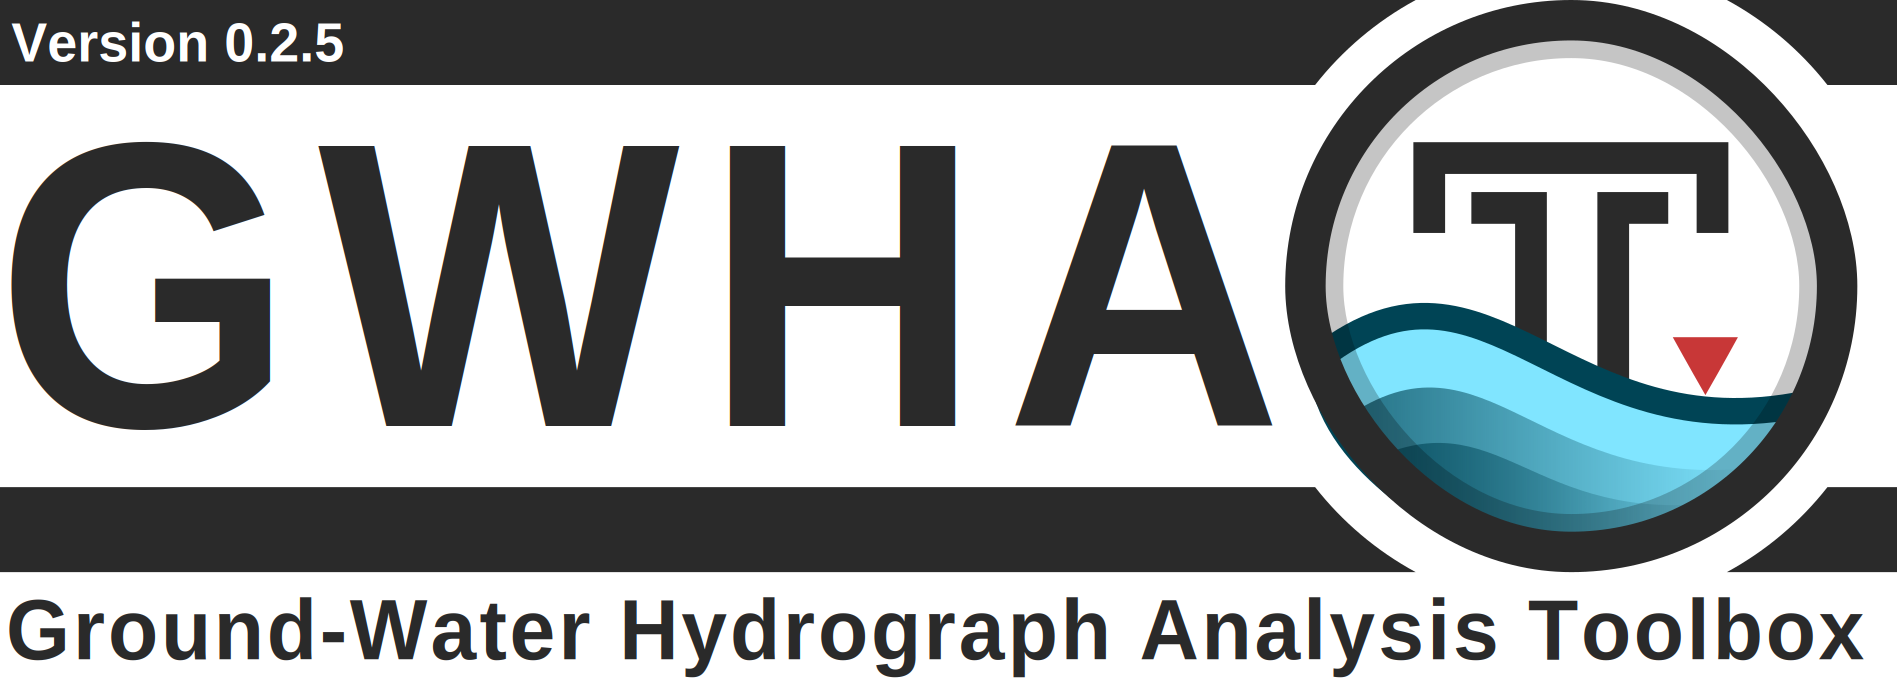
\includegraphics[width=1\textwidth]{WHAT_banner}~\\[2cm]

{\Large \today}\\[0.5cm]
{\Large Document up to data  for software version 4.1.5-beta}\\[2cm]

{\large Jean-S\'ebastien Gosselin\textsuperscript{1}, Christine Rivard\textsuperscript{2}, and Richard Martel\textsuperscript{1}}\\[0.25cm]

\textit{{\small\textsuperscript{1} Institut national de la recherche scientifique, Centre Eau Terre Environnement, 490 rue de la Couronne, Quebec City, Quebec, Canada}}\\[0.1cm]

\textit{{\small\textsuperscript{2} Geological Survey of Canada, Quebec Division, 490 rue de la Couronne, Quebec City, Quebec, Canada}}\\[2cm]

{Copyright 2015 Jean-S\'ebastien Gosselin}

\end{center}
\end{titlepage}


\chapter*{License}

WHAT is free software: you can redistribute it and/or modify it under the terms of the GNU General Public License as published by the Free Software Foundation, either version 3 of the License, or (at your option) any later version.

This program is distributed in the hope that it will be useful, but WITHOUT ANY WARRANTY; without even the implied warranty of MERCHANTABILITY or FITNESS FOR A PARTICULAR PURPOSE. See the GNU General Public License for more details.

You should have received a copy of the GNU General Public License along with this program. If not, see \url{www.gnu.org/licenses}.

\newpage

\chapter*{Acknowledgements}

WHAT has been funded in part by:

\begin{description}
\item{CRSNG through a PhD grant to Jean-Sébastien Gosselin}
\item{Projet Montérégie Est PACES}
\item{CRSNG fund}
\item{CGC}
\end{description}

We would like to thank all people who have used WHAT since its earliest stages and provided essential technical feedback, constructive criticism, and helpful comments or have helped in the shaping of the science that lies under the hood of the software. In particular, special thanks to (in alphabetical order):

\begin{description}
\item{Erwan Gloaguen, Professor of Geophysics and Geostatistics, INRS-ETE, Quebec, QC, Canada.}
\item{Harold Vigneault, Research Professional, INRS-ETE, Quebec, QC, Canada.}
\item{Marc Laurencelle, PhD Student in Earth Sciences, INRS-ETE, Quebec, QC, Canada.}
\item{Pierre Ladev\`eze, PhD Student in Earth Sciences, INRS-ETE, Quebec, QC, Canada.}
\item{Ren\'e Lefebvre, Professor in Hydrogeology, INRS-ETE, Quebec, QC, Canada.}
\item{Xavier Mallet, Research Technician, Geological Survey of Canada – Quebec Division, QC, Canada.}
\end{description}

\newpage

\chapter*{Introduction}

WHAT (Well Hydrograph Analysis Toolbox) is a free, open source, and cross-platform interactive computer program whose main focus is the interpretation of observation well hydrographs, including:

\begin{itemize}

\item{the preparation of a gapless daily weather time-series (precipitation and air temperature) representative of the well location. For this purpose, an interface to the online Canadian Daily Climate Database (CDCD) is provided that allows to query stations interactively by location coordinates, download the available data, and automatically rearranged the data in a format compatible with WHAT. Furthermore, missing data for a given station can be quickly filled with data from selected neighboring weather stations using a multiple linear regression model;}

\item{the generation of various publication-quality figures from the weather and water level data;}

\item{the exploration, manipulation, and validation of the data within a user-friendly dynamic graphical environment;}

\item{the calculation of the master recession curve of the well hydrograph (experimental);}

\item{the estimation of groundwater recharge at the local scale in unconfined conditions with a method combining the daily meteorological data and the water level time series (will be available in a future release).}

\item{the calculation of the barometric response function of the well that can be used to assess the level of confinement of the aquifer at the well location (will be available in a future release).}

\end{itemize}

WHAT is written in the Python 2.7 programming language and is currently maintained and developed by Jean-Sébastien Gosselin at INRS-ETE (\url{www.ete.inrs.ca}). The source code and a stand-alone executable for Windows 7 are available free of charge for download on GitHub (\url{https://github.com/jnsebgosselin/WHAT}). If you encounter any problems or errors during program execution, have any questions, or have specific suggestions on how to improve WHAT, please contact Jean-Sébastien Gosselin at this email address \href{mailto:jnsebgosselin@gmail.com}{jnsebgosselin@gmail.com}.

\listoffigures

\tableofcontents

\chapter{User Manual}

\section{Installation}\label{sec:intallation}

WHAT can run on Windows, Linux, or OS X computer operating systems. However, a stand-alone executable of the program is currently released and tested only for the Windows 7 platform. This executable should also be compatible with Windows XP. For the Linux and OS X platforms, the software can be run directly from the source code, provided that Python 2.7 and all the required third party packages are installed on the computer (PySide, NumPy, matplotlib, xlrd, xlwt).

The stand-alone executable for Windows 7 is distributed in a Zip archive that can be downloaded freely on GitHub (\url{https://github.com/jnsebgosselin/WHAT/releases}). This archive contains:

\begin{itemize}

\item{the GNU General Public License;}

\item{a folder named ``WHAT'' that contains all the necessary system files for the program to run, including the file ``WHAT.exe'' from which the software can be started;}

\item{a folder named ``Projects'' where all input and output files used or created by WHAT are stored by default. In this folder are included samples of input and output files that provide a quick and convenient way to test and learn the various features of the program.}

\end{itemize}

Once the content of the Zip archive has been extracted, the program can be started directly from the WHAT.exe executable file that is contained withing the folder named WHAT. The software can conveniently run from any location on the computer or from any storage device without the need to install the program beforehand.

\section{Overview of the Graphical User Interface}

WHAT Graphical User Interface (GUI) mainly consists of a menu bar, a console area, and a central view panel (see Figure 1). The menu bar is located in the top right corner of WHAT main window. This is where you can view and edit the current project directory. The project directory is a folder location where all the input, output and parameter files associated with a given project are gathered. For more information about the project directory content and files organization, please refer to section 2.3.2. When opening WHAT for the first time, the current project is setup by default to an example that is provided with the software with the necessary files to test all the functionalities of the program. The console is located at the bottom of the main window and is used to report technical information about the various tasks accomplished by the program as well as warning and error messages. The console can be completely collapsed to save space, or can be fully expanded to the entire area of the window. The central view panel is equipped of a tab bar at the top where you can navigate through the various functionalities of the program. There is a total of four tabs available: Download Data, Fill Data, Hydrograph, and About. The tabs are described in a little bit more details in the text below and are also presented in Figures 2 to 5.

The Download Data tab (Figure 2) provides an interface to the online Canadian Daily Climate Database (CDCD) that allows to query stations interactively by location coordinates, download the available data, and automatically rearranged the data in a format compatible with WHAT. Alternately, it is possible to provide a custom list of Canadian weather stations for which data can be downloaded and formatted. At the moment, it is not possible to access data of weather stations located in the U.S. This feature may be added in a future release of the software.

The Fill tab (see Figure 3) is where you can automatically estimate the missing daily weather values in your data to create gapless time-series of daily precipitation and air temperature. Missing data for a given station are estimated from selected neighboring weather stations using a multiple linear regression model;

The Hydrograph tab is used for viewing and plotting data. For this purpose, two modes are available: the layout and the computation mode. Both modes share the same weather and water level dataset. It is possible to switch from one mode to the other at anytime. The layout mode (see Figure 4) provides an interface to interactively produce publication-quality graphs from the data. The computation mode (see Figure 5) consists in a dynamic graphical environment where data can be explored, manipulated and analyzed. Various computation tools are available in this mode, including the estimation of the hydrograph Master Recession Curve (MRC) and the estimation of groundwater recharge.

The About tab displays copyright, licensing and general information about WHAT.

\section{Interpretation of water-level time-series with WHAT}

\subsection{Introduction}

WHAT essentially consists of set of tools to assist the interpretation of water level time series measured in observation wells, from the preparation of raw data to the assessment of groundwater recharge when in unconfined conditions. In this perspective, WHAT was developed with the general workflow shown in Figure 6  in mind.

The first step consists in the preparation of a gapless weather dataset.

Validation/preparation of water level time series: 1) automatic measurements fitted to manual measurements. 2) Correct the places where there is a break in the water level curve. This is due generally to the logger that is placed at a different level following the removal of the later from the well. 3) Remove measurements that were acquired while the barologger was outside the water column.

Preparation of a gapless weather dataset. This include. Downloading data from the CDCD database for stations located in a radius of 0 to 100 km from the well. Fill missing daily data for the station located closest to the well by using selected neighboring stations. Data are not interpolated to the exact location of the well. It has been decided to keep the original dataset of the station located closest to the well to analyse the data. This is due to the fact that conventional technique for interpoloating weather data tend to surestimate the number of wet day, but underestimate the intensity of stron precipitation event. More advanced and complicated technique are required to circumvent these issues. It has thus been decided that is was prefereable to keep the original data from a single station.

Once the weather data, and water level are prepared, production of a well hydrograph. Visual interpretation between the water level  fluctuation and weather data can be done.

If high time resolution measurement of the water level and barometric pressure are available, it is possible to carry an calculation of the barometric response function. It is also good to produce a FFT analysis of the hydrograph.
Weather yearly average and montlhy averages can be plotted at this stage.
If the visual inspection of the well, and the barometric response function, determined that the well in unconfined, it means groundwater recharge can be estimated from the data. First, determining the segment where groundwater recharge can be supposed to be negligible and where the water level recede. After that, compute the MRC, and compute a first estimation of groundwater recharge using the Water-Table Fluctuation principle. Estimate finaly recharge with a method combining the meteorological data and the well hydrograph. Enjoy.

\subsection{New and Open Project}

Data is managed in WHAT by project. That is all input and output files relative to a given project are saved within a common folder called the ``project folder''. This file management system allows you to easily backup and move your projects from one location to the other since all the files relating to a same project are saved at the same location.

\begin{figure}[h!]
\centering
\includegraphics[width=0.5\textwidth]{WHAT_Screenshot_newproject}
\caption[New Project dialog window.]{New Project dialog window.}
\label{fig:new_proj_win}
\end{figure}

By default, the current active project is setup to an example that is distributed with the software. To start a new project, click on the \textsl{New Project\dots} button located at the right end of the WHAT menu bar (see Figure~X). This will open a new dialog window (see Figure~\ref{fig:new_proj_win}) where you can enter various information about your project such as its title, author and location coordinates. Clicking on the \textsl{Save} button will save your project in a folder named after your project title in the location defined by the \textsl{Save in Folder} directory path. For example, the \textsl{My New Project} of Figure~\ref{fig:new_proj_win} would be saved by default in a folder named ``My New Project'' in the directory ``\textsl{C:\textbackslash{}Users\textbackslash{}johndoe\textbackslash{}WHAT\_4.0.5-beta\textbackslash{}Projects}''. You can change the directory where your project is saved by default by clicking the small folder icon located next to the \textsl{Save in Folder} directory path.

% Add a comment about relative link here

%%Path to your project folder is stored in WHAT in a relative format. This means that if you change the location of your project folder relative the ``WHAT.exe'', your will have to redirect WHAT to the new location of your project folder.

When a new project is saved, WHAT automatically creates within the project folder the predefined file organization that is presented in Figure~\ref{fig:proFolder_organization}.

In this example, we have the project My New Project, that is located within the folder Projects within the folder that contain the program.

\begin{figure}[h!]
\centering
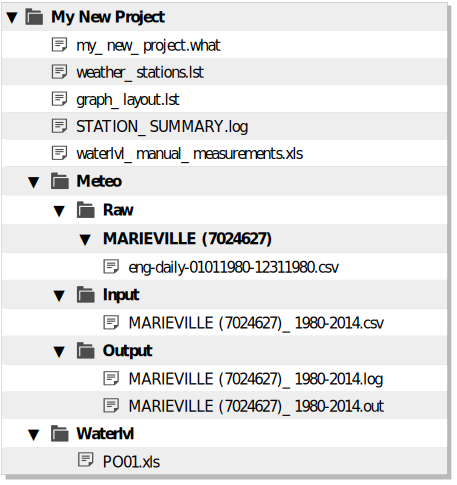
\includegraphics[width=0.5\textwidth]{file_and_folder_architecture}
\caption[Project folder file organization.]{Project folder file organization.}
\label{fig:proFolder_organization}
\end{figure}

\section{Creation of gapless weather data serie}

The view can be panned by dragging the mouse with the left mouse button depressed. Zoom in by pressing the Ctrl key while dragging the mouse upwards, or by moving the mouse wheel up. Zoom out mouse wheel down.

The Canadian Daily Climate Database (CDCD) contains daily temperature, precipitation and snow on the ground data for almost 8000 locations in Canada. Green Kenue provides a graphical interface to the CDCD database with which you can query, display, and analyze the data associated with each station

by clicking on the Toggle button located at the left end of the toolbar

\subsection{Downloading and formatting data from the CDCD database}

Daily meteorological records are made available free of charge by the Government of Canada from 1840 to the present for about 8450 stations distributed across Canada (www.climate.weather.gc.ca). Record length and availability of data vary widely among these stations. Meteorological data for a given station can be downloaded manually on the Government of Canada website for each year separately as a CSV file, or it is possible to acquire the entire dataset by ordering a DVD. However, this involves a lot of repetitive manipulations and can become quickly a time consuming task when meteorological data are required for several stations over many years. Moreover, the pooling of individual data files downloaded for each year separately is also a tedious task when done manually.

Rainbird alleviate this process by allowing automatic downloading and formatting of daily meteorological records from the Government of Canada website. This feature is explained in more detail in the following sections.

The first step consists in producing a file containing a list of weather station names along with their corresponding unique Station ID, the first and last year for which data are available and the province where they are located. All this information can be retrieved for a given station directly from its unique URL on www.climate.weather.gc.ca. An example for the weather station Marieville, located in southern Quebec, is presented in Appendix A.

The stations' information need to be saved in a tabular-separated values text file with an “lst” extension. A template of a station list (station\_list\_template.lst) is provided with the program in the Zip archive and an example is presented in Error: Reference source not found. The fields Station Name, Year, Start, Year End and Province do not need to match strictly with the station's URL. These fields can be assigned any name/value by the user and are not directly used in the downloading process of weather data. The only field that is directly used in the download process is Station ID that is a unique number attributed to each weather station.

Once a file containing a list of weather stations' information has been created, it is possible to load it in Rainbird by clicking on the  Load button located in the Fetch and Merge tab (Error: Reference source not found). The station list can be refreshed at any time by clicking on the  Refresh button. 
After a list has been loaded in Rainbird, a weather station can be selected from the drop-down menu Station name. The fields Station ID and Years will automatically display the information that are related to the selected weather station. The Station ID is a number that is unique for each station and cannot be changed. Conversely, the lower and upper limits for the Years can be set to any value, including years where there is no data available for the selected station. 

The downloading of raw data is started by clicking on the  Fetch button. It is possible to stop the downloading process at any time by clicking again on the same button. Meteorological data are downloaded for every available year between the values specified in the Years limits and saved in CSV (comma-separated values) files for each year separately (note that this is a limitation imposed by the Government of Canada website). These CSV data files, hereafter referred to as Error: Reference source not found, are saved automatically in the current Target Directory that corresponds by default to the Raw folder located in the Error: Reference source not found. For years with no data, Rainbird will generate a raw data file with empty values everywhere.

When a downloading process is completed successfully, statistics regarding the amount of missing data for the entire dataset downloaded are displayed. The statistics provide information on the number of missing data for each meteorological variable over the entire selected record. The amount of missing values is also given in percentages, in parentheses.

As soon as a downloading process is completed successfully for a given weather station, Rainbird automatically format and concatenate the entire dataset that was downloaded for each year separately. That is data for each year are put together end to end in chronological order. In addition, the program will automatically detect and put a NaN value wherever a data is missing. The resulting data series can be subsequently saved in a single CSV file, hereafter called a Error: Reference source not found, by clicking on the   Save button. Concatenated data files thus generated can be used directly as input for the estimation of missing data and the completion of meteorological series (gap filling procedure) in Rainbird. An example of a concatenated data file is presented in Figure 1.

It is possible to reload previously downloaded Error: Reference source not found in Rainbird at any time by clicking on the  Select button. Rainbird will then automatically format and concatenate the data and a new concatenated data files can be saved by clicking on the  Save button. This feature is useful to update meteorological records without having to download previously downloaded data a second time.

The process of saving concatenated data files can also be made automatic, after a downloading process is completed successfully or after previously downloaded raw data files have been loaded manually in Rainbird, by checking Automatically save concatenated data in “Merge” folder.

\subsection{Use of weather data from other sources}

Automatic downloading and formatting of weather data from other sources than the Government of Canada is currently not supported in Rainbird. However, it is possible to use weather data from any sources for the gap filling procedure of meteorological records, as long as data are formatted as follows. A template of a typical Error: Reference source not found is provided with the program within the Zip archive in the Merge folder and an example is presented in Figure 1.

Data must be tab-separated and saved in a file with a csv extension. This can be easily achieved in any standard spreadsheet application such as Microsoft Excel or LibreOffice Calc (www.libreoffice.org). The format of the header must be observed faithfully (see example in Figure 1). NaN values must be inputted where data are missing. Data must also be in chronological order, but do not need to be continuous over time. That is missing blocks of data (e.g., several months or years) can be completely omitted in the concatenated data file. These missing blocks of data will be estimated and filled during the gap filling procedure.

\subsection{Gap filling daily weather records}

Rainbird main feature consists in an automatic gap filling procedure of weather data records. This feature is accessible from the tab Fill (Error: Reference source not found). In order to fill gaps in a meteorological dataset for a given station, herein called the Error: Reference source not found, Rainbird needs data from at least one Error: Reference source not found with synchronous data.

This is achieved by first selecting the Data directory where are stored the Error: Reference source not found for the weather stations located in a given study area. The default folder used by the program is the Merge folder located in the Error: Reference source not found. This folder is the default location where are saved the concatenated data files produced by Rainbird from data downloaded on the Government of Canada website.

Rainbird scans automatically the default Data directory for valid concatenated data files at startup and displays the result in the drop-down menu Target station. If a new Data directory is selected by the user with the  Browse button, Rainbird scans its content automatically. The  Refresh button can also be used at any time to scan the Data directory again for new concatenated data files.

As soon as a weather station is selected from the drop-down menu, Rainbird calculates correlation coefficients between the target station's meteorological time series and those of each neighboring station. It also calculates differences in altitude and horizontal distances between the target station and every other station.

By default, correlation coefficients that fall below a value of 0.7 are displayed in red in the table. This is only meant as guidance for the user and has no impact on the gap filling procedure. For each missing data in the target station's meteorological time series, Rainbird estimates a value using data available from the neighboring stations that are best correlated with data from the target station, up to the maximum number of stations defined by the user. For example, in Error: Reference source not found, the program would use the neighboring stations with the best correlation coefficient values up to a maximum of four. It is possible that for a given date, neighboring stations may all have missing data, synchronously with the target station. In this case, the missing data at this particular date cannot be estimated and a NaN value is kept within the original dataset.

Generally, data correlation between two stations for a given meteorological variable will decreases as difference in altitude and distance increase. Thereby, it is also possible to specify a cutoff distance and a cutoff altitude difference for which neighboring stations that fall above these cutoff values are excluded from the gap filling procedure. A value of 100 km for the cutoff distance and 350 m for the cutoff altitude difference are set as default values in the program, based on the literature (Tronci et al., 1986; Xia et al., 1999; Simolo et al., 2010).

More specifically, missing data in the target station's dataset are estimated using a multiple linear regression model that is generated between the synchronous target station and the neighboring stations meteorological time series. It has been demonstrated that multiple linear regression method outperforms most of the commonly used techniques for the estimation of missing data in daily meteorological records (Eischeid et al., 1995, 2000; Xia et al., 1999). In addition, the user can choose between a regression model that is generated using either an Ordinary Least Squares (OLS) or a Least Absolute Deviations (LAD) criterion. LAD is more robust to outliers than OLS but is more demanding in computation time.

Once the parameters are set as desired, the gap filling procedure can be started by clicking on the        Fill and Save button. The process can be stopped at any time by clicking on the same button a second time. When all the gaps in the target station's dataset have been filled, the gapless meteorological time series are saved automatically in a new Error: Reference source not found named <target station name>.csv in the folder Output located in the Error: Reference source not found, along with an Error: Reference source not found named <target station name>.log. The info file provides a list of all the missing meteorological values that were estimated during the gap filling procedure, along with their associated date, and neighboring stations data values that were used for the estimation. An estimation of the uncertainty for each value estimated is also given.

\section{Preparation of the water level time series}

\subsection{Data validation and correction}

Pour chacun des puits, les valeurs de niveaux d’eau obtenues avec les sondes ont été comparées avec des mesures manuelles prises lors des visites aux puits. Pour l’ensemble des puits, l’écart absolu entre les valeurs des sondes et les mesures manuelles est généralement inférieur à 5 cm.

Pour un même puits, lorsqu'un écart systématique de plus de 5 cm était observé entre les mesures manuelles et les mesures automatiques, une correction des niveaux d’eau a été  appliquée de façon à caler les valeurs obtenues avec les sondes aux mesures manuelles.
Les données aberrantes dans les séries de données ont également été corrigées par interpolation linéaire. C’est données aberrantes sont principalement des mesures qui ont été prises alors que la sonde avait été retirée du puits pour le téléchargement des données, ou encore par du pompage dans les puits lors d’une campagne d’échantillonnage de l’eau.

\subsection{Generation of the well hydrograph with weather data}
\subsection{Barometric response function}
\subsection{Estimation of the MRC and first recharge estimation}
\subsection{Recharge estimation with synthetic well hydrograph method}

\chapter{Technical Documentation}

\section{Barometric correction: an overview}

Even though there exists software that can correct the data automatically, it is always a good practice to understand what is done behie. This is particularly usefull to correct situations when something goes wrong. For example, the barologger may had a deficiency and atmospheric pressure needed to be taken from the CDCD for example and data needed to be corrected manually. There arise often situation when correction needs to be done manually. This happens when there is a problem with the data. This is then good practice to understand the process in order to dodge mistake.

It is a good idea to monitor water level at a 15 min frequency for a period of a year, or more if it is possible. The data can be used subsequently to estimate the barometric response function of the well that can be quite usefull to understand the hydrogeological context, and the level of confinement of the well. Having data with this frequency is also usefull for running FFT and understand the cause of possible unatural fluctuation in the well. 

Figure 2: Schématisation de la configuration des instruments pour le monitoring des puits

\subsection{Format des données brutes}

Le monitoring des niveaux d’eau dans les puits d’observation pour le projet Montérégie Est a été fait avec des sondes à niveaux d’eau non ventilées. Cela implique que pour pouvoir calculer la hauteur de la colonne d'eau, heau, située au-dessus des sondes (voir figure 1), la pression atmosphérique doit également être connue à chacun des puits. À cet effet, des sondes barométriques ont également été installées dans la majorité des puits d'observation du projet Montérégie Est. Une attention particulière a été portée afin d'assurer que les puits qui n'étaient pas munis d'une sonde barométrique étaient situés à proximité et à une altitude raisonnablement similaire d'un puits où la pression atmosphérique était mesurée.

De façon générale, la profondeur de la nappe par rapport à la surface, Znappe, est calculée via l'équation suivante : 

où Znappe (m) et Zsonde (m) correspondent respectivement à la position de la nappe et la profondeur d'installation de la sonde à niveaux d'eau par rapport à la surface du sol, htot (m) est la charge totale mesurée par la sonde à niveaux d'eau et hatm (m) est la charge mesurée par la sonde barométrique. L'axe des z est défini positif vers le haut avec, pour niveau de référence, la surface du sol. Ainsi Zsonde et Znappe ont des valeurs qui sont généralement inférieures à zéro, à moins que le niveau de l'eau dans le puits ne soit situé au-dessus de la surface.

Au cours du projet, trois modèles de sondes ont été utilisés pour la mesure des niveaux d’eau: (1) levelogger Gold de Solinst, (2) levelogger Edge de Solinst et (3) Micro-Diver de Schlumberger. Parallèlement, deux modèles de sondes ont été utilisés pour la mesure de la pression atmosphérique: (1) barologger Gold de Solinst et (2) barologger Edge de Solinst. Il est important de savoir que la méthode de stockage des données brutes varie d'un instrument à l'autre. C’est-à-dire que des transformations mathématiques sont parfois appliquées sur les mesures avant de les mettre en mémoire. En général, cela ne cause pas de problème car les logiciels de traitement des données fournis par les fabricants gèrent le tout de façon automatique et implicite. Par contre, lorsqu'une manipulation manuelle des données brutes est nécessaire ou lorsque des analyses plus complexes sont envisagées, une connaissance des différentes stratégies de stockage des instruments est essentielle.
Pour les sondes levelogger et barologger Gold, les données brutes enregistrées par les instruments correspondent aux pressions mesurées, converties en hauteur d'eau équivalente, moins une constante dont la valeur est établie en fonction de la pression atmosphérique minimale anticipée au niveau de la mer et de l'altitude fournie à la sonde par l'utilisateur lors de sa programmation (9.5 m - 0.0012 m par mètre d'altitude). Pour les sondes Micro-Diver et Levelogger Edge, les données brutes enregistrées par les instruments correspondent aux pressions mesurées converties en hauteur d'eau équivalente. Enfin, pour les sondes barologger Edge, la pression atmosphérique est directement mise en mémoire sans aucune transformation préalable. Le Tableau 1 résume les différentes opérations mathématiques qui sont appliquées aux mesures avant de les mettre en mémoire pour les différents types de sondes qui furent utilisées au cours du projet Montérégie.

où Ptot (kPa) est la pression absolue ressentie par la sonde à niveaux d'eau, Patm (kPa) est la pression atmosphérique, ρ (kg/m3) est la masse volumique de l'eau, g (m/s2) est l'accélération gravitationnelle terrestre et Zalt (m) est l'altitude du puits fourni à la sonde par l'utilisateur lors de sa programmation.


\end{document}